\section{Experiments and Results}
TODO
\subsection{Frequent Words}
Ben
\subsection{Sentiment Analysis}
For each community, we calculated the percentage of positive, neutral, and negative posts from all community posts, these results can be found in Figure~\ref{fig:Polarity} below. It can be seen that in all communities most posts are extreme, positive or negative and less neutral.
Additionally, we calculate the positive and negative polarity values average for every community, these results can be found in Figure~\ref{fig:PolarityAverage}.

\begin{figure}[h]
    \begin{center}
        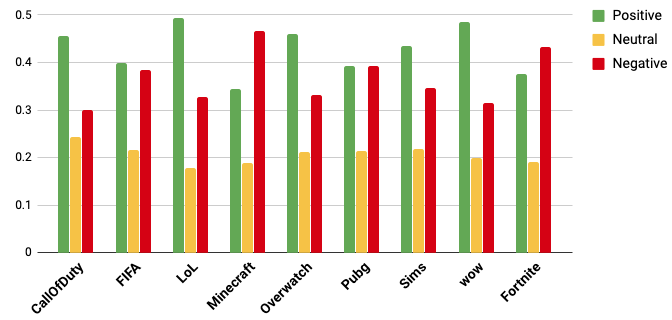
\includegraphics[scale=0.32]{Images/Polarity.png}
    \end{center}
    \caption{The X-axis shows the communities, the Y-axis present the percentage of positive/ neutral/ negative posts according to the appropriate series. For example, 40 percent of the posts in the FIFA community had positive polarity.}
    \label{fig:Polarity}
\end{figure}

\begin{figure}[h]
    \begin{center}
        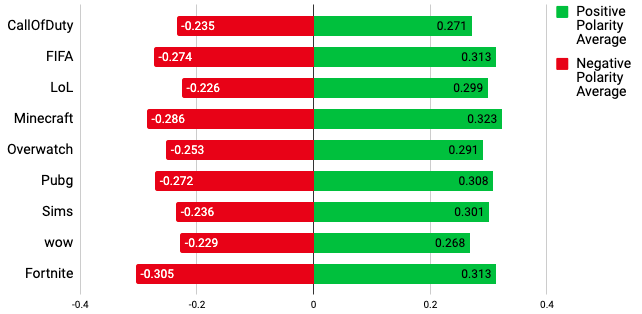
\includegraphics[scale=0.32]{Images/PolarityAverage.png}
    \end{center}
    \caption{The Y-axis shows the communities, the X-axis present the polarity average value. For example, the average score of posts with positive polarity was 0.313 in FIFA community, and the negative polarity average score was -0.274 at the same community.}
    \label{fig:PolarityAverage}
\end{figure}

\subsection{Word Embedding}
Julia
\subsection{Negativity Evaluation Metric}
Yuval


